\documentclass[11pt, a4paper]{article}\usepackage[]{graphicx}\usepackage[]{xcolor}
% maxwidth is the original width if it is less than linewidth
% otherwise use linewidth (to make sure the graphics do not exceed the margin)
\makeatletter
\def\maxwidth{ %
  \ifdim\Gin@nat@width>\linewidth
    \linewidth
  \else
    \Gin@nat@width
  \fi
}
\makeatother

\definecolor{fgcolor}{rgb}{0.345, 0.345, 0.345}
\newcommand{\hlnum}[1]{\textcolor[rgb]{0.686,0.059,0.569}{#1}}%
\newcommand{\hlsng}[1]{\textcolor[rgb]{0.192,0.494,0.8}{#1}}%
\newcommand{\hlcom}[1]{\textcolor[rgb]{0.678,0.584,0.686}{\textit{#1}}}%
\newcommand{\hlopt}[1]{\textcolor[rgb]{0,0,0}{#1}}%
\newcommand{\hldef}[1]{\textcolor[rgb]{0.345,0.345,0.345}{#1}}%
\newcommand{\hlkwa}[1]{\textcolor[rgb]{0.161,0.373,0.58}{\textbf{#1}}}%
\newcommand{\hlkwb}[1]{\textcolor[rgb]{0.69,0.353,0.396}{#1}}%
\newcommand{\hlkwc}[1]{\textcolor[rgb]{0.333,0.667,0.333}{#1}}%
\newcommand{\hlkwd}[1]{\textcolor[rgb]{0.737,0.353,0.396}{\textbf{#1}}}%
\let\hlipl\hlkwb

\usepackage{framed}
\makeatletter
\newenvironment{kframe}{%
 \def\at@end@of@kframe{}%
 \ifinner\ifhmode%
  \def\at@end@of@kframe{\end{minipage}}%
  \begin{minipage}{\columnwidth}%
 \fi\fi%
 \def\FrameCommand##1{\hskip\@totalleftmargin \hskip-\fboxsep
 \colorbox{shadecolor}{##1}\hskip-\fboxsep
     % There is no \\@totalrightmargin, so:
     \hskip-\linewidth \hskip-\@totalleftmargin \hskip\columnwidth}%
 \MakeFramed {\advance\hsize-\width
   \@totalleftmargin\z@ \linewidth\hsize
   \@setminipage}}%
 {\par\unskip\endMakeFramed%
 \at@end@of@kframe}
\makeatother

\definecolor{shadecolor}{rgb}{.97, .97, .97}
\definecolor{messagecolor}{rgb}{0, 0, 0}
\definecolor{warningcolor}{rgb}{1, 0, 1}
\definecolor{errorcolor}{rgb}{1, 0, 0}
\newenvironment{knitrout}{}{} % an empty environment to be redefined in TeX

\usepackage{alltt}

\usepackage[top=1 in, bottom = 1 in, left = 1 in, right = 1 in ]{geometry}

\usepackage{amsmath, amssymb, amsfonts}
\usepackage{enumerate}

\title{003 A Detailed Example}
\author{Ananda Biswas}
\date{}
\IfFileExists{upquote.sty}{\usepackage{upquote}}{}
\begin{document}

\maketitle

\begin{figure}[h]
	\centering
	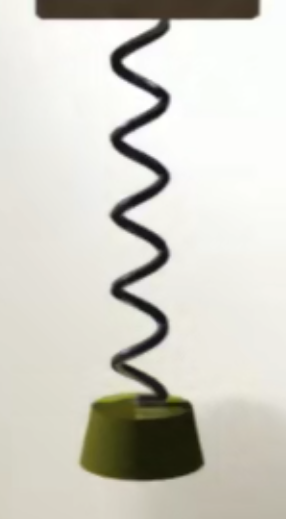
\includegraphics[scale = 0.35]{Screenshot (1473)}\\
\end{figure}

\begin{figure}[h]
	\centering
	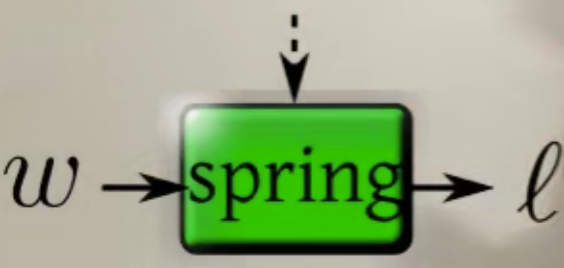
\includegraphics[scale = 0.35]{Screenshot (1474)}\\
\end{figure}

Once we have the blackbox, we shall take multiple instances of the object, depending on the system we are working on.\\
Here we shall take multiple such springs. If the blackbox were patient, we would have taken multiple patients. \\
We have to make sure that the units(springs, patients) are as identical as possible. Some amount of variation will be there, that will be considered as part of random error, but we shall try to keep that as small as possible.\\

\begin{figure}[h]
	\centering
	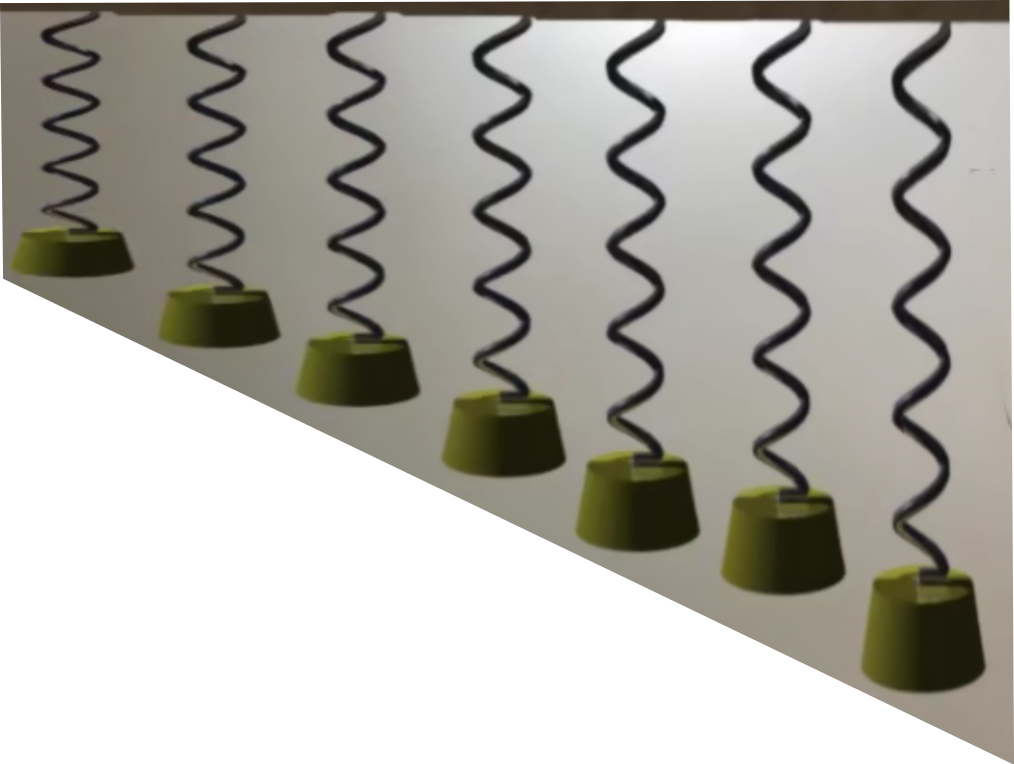
\includegraphics[scale = 0.15]{download}\\
\end{figure}

We are giving different weights(inputs) to the springs and for each of the cases we are measuring the length of the spring. \\
Here we have a covariate(as input weight $w$ is continuous) and a continuous output length $l$.\\

Now we shall write our model, the mathematical formulation of the system. \\

$$l = \beta_1 + \beta_2 w + \epsilon$$

$\beta_1$ and $\beta_2$ are unknown constants, they are common properties of the identical strings.\\

Here we are expressing the output $l$ as a linear function of input $w$ and random error $\epsilon$.\\

For $n$ instances of the object, we shall have $$l_i = \beta_1 + \beta_2 w_i + \epsilon_i, \hspace{10pt} \forall \hspace{3pt} i = 1, 2, 3, \ldots n.$$

Converting our model in matrix form, we shall have,
\begin{gather}
	\begin{bmatrix} l_1 \\	l_2 \\	\vdots \\	l_n	\end{bmatrix}
	=
	\begin{bmatrix}	1 & w_1 \\	1 & w_2 \\	\vdots & \vdots \\	1 & w_n	\end{bmatrix} 
	\cdot
	\begin{bmatrix}	\beta_1 \\	\beta_2 \\	\end{bmatrix}  
	+	
	\begin{bmatrix}  \epsilon_1 \\	\epsilon_2 \\	\vdots \\	\epsilon_n	\end{bmatrix}.
\end{gather}

$ \begin{bmatrix}	1 & w_1 \\	1 & w_2 \\	\vdots & \vdots \\	1 & w_n	\end{bmatrix} $ is the \textbf{design matrix} $i.e.$ it is designed by us, we exactly know the weights $w_i$s that we gave as inputs.

\begin{knitrout}
\definecolor{shadecolor}{rgb}{0.969, 0.969, 0.969}\color{fgcolor}\begin{kframe}
\begin{alltt}
\hldef{our_data} \hlkwb{=} \hlkwd{read.csv}\hldef{(}\hlsng{"springs.csv"}\hldef{)}

\hldef{our_data}
\end{alltt}
\begin{verbatim}
##   weight length
## 1    1.0   5.29
## 2    1.5   6.31
## 3    2.0   7.28
## 4    2.5   8.33
## 5    3.0   9.30
## 6    3.5  10.32
\end{verbatim}
\begin{alltt}
\hlkwd{dim}\hldef{(our_data)}
\end{alltt}
\begin{verbatim}
## [1] 6 2
\end{verbatim}
\end{kframe}
\end{knitrout}

\begin{knitrout}
\definecolor{shadecolor}{rgb}{0.969, 0.969, 0.969}\color{fgcolor}\begin{kframe}
\begin{alltt}
\hlkwd{plot}\hldef{(length} \hlopt{~} \hldef{weight,} \hlkwc{data} \hldef{= our_data)}
\end{alltt}
\end{kframe}
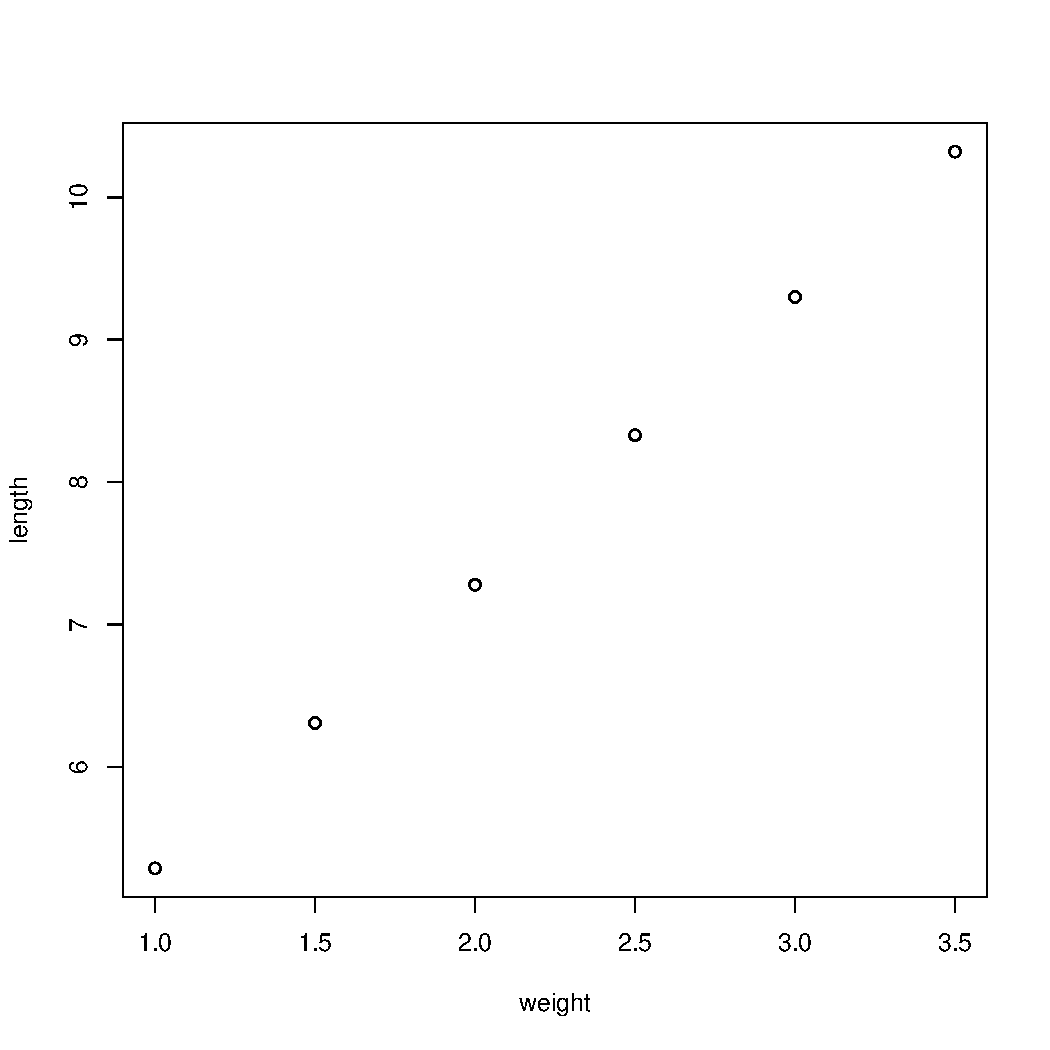
\includegraphics[width=\maxwidth]{figure/unnamed-chunk-2-1} 
\end{knitrout}

\begin{knitrout}
\definecolor{shadecolor}{rgb}{0.969, 0.969, 0.969}\color{fgcolor}\begin{kframe}
\begin{alltt}
\hldef{fit} \hlkwb{=} \hlkwd{lm}\hldef{(length} \hlopt{~} \hldef{weight,} \hlkwc{data} \hldef{= our_data)}
\end{alltt}
\end{kframe}
\end{knitrout}

\begin{knitrout}
\definecolor{shadecolor}{rgb}{0.969, 0.969, 0.969}\color{fgcolor}\begin{kframe}
\begin{alltt}
\hlkwd{model.matrix}\hldef{(fit)}
\end{alltt}
\begin{verbatim}
##   (Intercept) weight
## 1           1    1.0
## 2           1    1.5
## 3           1    2.0
## 4           1    2.5
## 5           1    3.0
## 6           1    3.5
## attr(,"assign")
## [1] 0 1
\end{verbatim}
\end{kframe}
\end{knitrout}

\begin{knitrout}
\definecolor{shadecolor}{rgb}{0.969, 0.969, 0.969}\color{fgcolor}\begin{kframe}
\begin{alltt}
\hldef{fit}
\end{alltt}
\begin{verbatim}
## 
## Call:
## lm(formula = length ~ weight, data = our_data)
## 
## Coefficients:
## (Intercept)       weight  
##       3.283        2.010
\end{verbatim}
\end{kframe}
\end{knitrout}

\begin{knitrout}
\definecolor{shadecolor}{rgb}{0.969, 0.969, 0.969}\color{fgcolor}\begin{kframe}
\begin{alltt}
\hlkwd{names}\hldef{(fit)}
\end{alltt}
\begin{verbatim}
##  [1] "coefficients"  "residuals"     "effects"       "rank"         
##  [5] "fitted.values" "assign"        "qr"            "df.residual"  
##  [9] "xlevels"       "call"          "terms"         "model"
\end{verbatim}
\end{kframe}
\end{knitrout}

\begin{knitrout}
\definecolor{shadecolor}{rgb}{0.969, 0.969, 0.969}\color{fgcolor}\begin{kframe}
\begin{alltt}
\hldef{fit}\hlopt{$}\hldef{coefficients}
\end{alltt}
\begin{verbatim}
## (Intercept)      weight 
##    3.283143    2.009714
\end{verbatim}
\end{kframe}
\end{knitrout}

\begin{knitrout}
\definecolor{shadecolor}{rgb}{0.969, 0.969, 0.969}\color{fgcolor}\begin{kframe}
\begin{alltt}
\hldef{fit}\hlopt{$}\hldef{residuals}
\end{alltt}
\begin{verbatim}
##            1            2            3            4            5            6 
## -0.002857143  0.012285714 -0.022571429  0.022571429 -0.012285714  0.002857143
\end{verbatim}
\end{kframe}
\end{knitrout}

\begin{knitrout}
\definecolor{shadecolor}{rgb}{0.969, 0.969, 0.969}\color{fgcolor}\begin{kframe}
\begin{alltt}
\hldef{fit}\hlopt{$}\hldef{fitted.values}
\end{alltt}
\begin{verbatim}
##         1         2         3         4         5         6 
##  5.292857  6.297714  7.302571  8.307429  9.312286 10.317143
\end{verbatim}
\end{kframe}
\end{knitrout}

\begin{knitrout}
\definecolor{shadecolor}{rgb}{0.969, 0.969, 0.969}\color{fgcolor}\begin{kframe}
\begin{alltt}
\hldef{fit}\hlopt{$}\hldef{rank}
\end{alltt}
\begin{verbatim}
## [1] 2
\end{verbatim}
\end{kframe}
\end{knitrout}

\begin{knitrout}
\definecolor{shadecolor}{rgb}{0.969, 0.969, 0.969}\color{fgcolor}\begin{kframe}
\begin{alltt}
\hlkwd{plot}\hldef{(length} \hlopt{~} \hldef{weight,} \hlkwc{data} \hldef{= our_data)}
\hlkwd{abline}\hldef{(fit}\hlopt{$}\hldef{coefficients)}
\end{alltt}
\end{kframe}
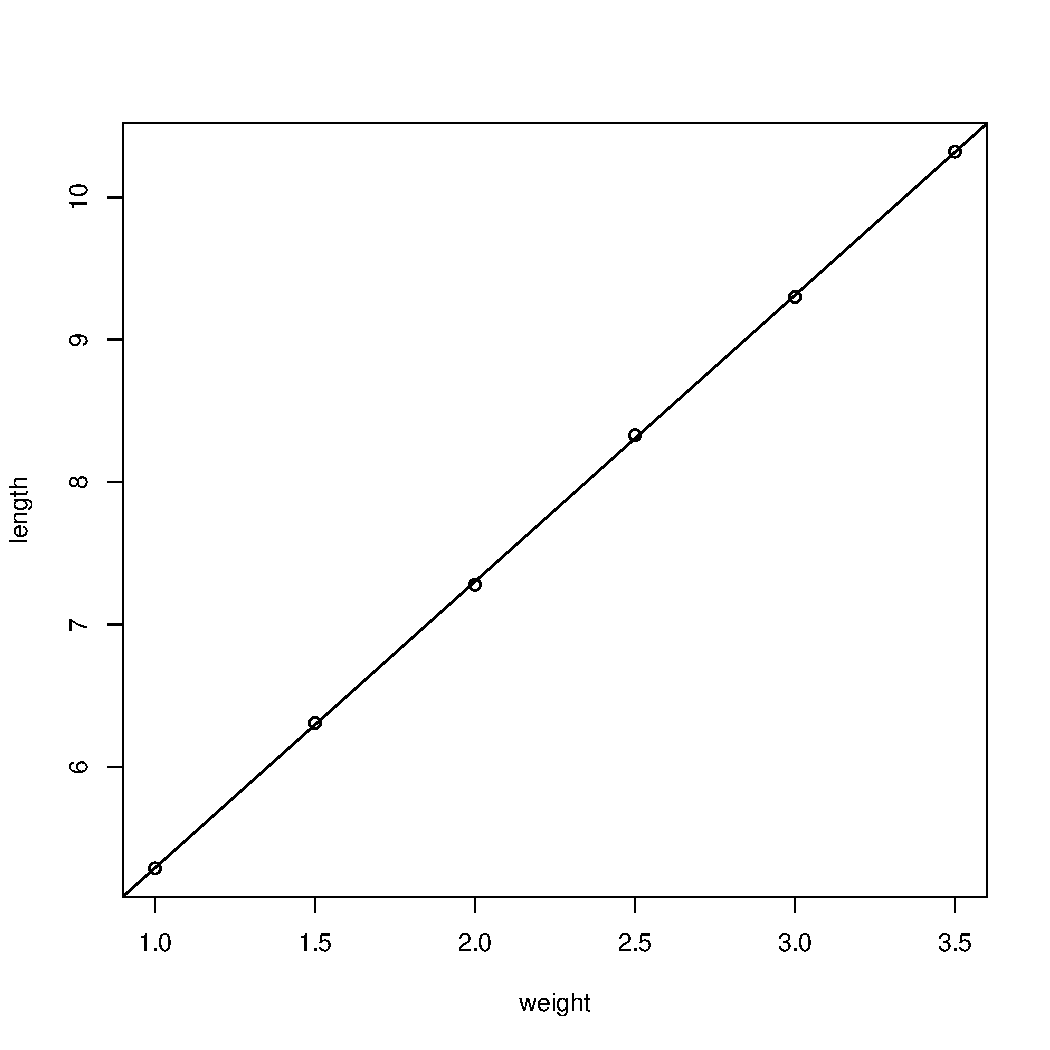
\includegraphics[width=\maxwidth]{figure/unnamed-chunk-11-1} 
\end{knitrout}

\section*{The Important Steps}

\begin{enumerate}[(1)]

\item Draw the blackbox

\item Make n sets of measurements

\item Create a CSV file. No. of columns = no. of inputs + 1. In the columns, we shall have the inputs and the output. No. of rows will be n.

\item Load the file in R.

\item Do some sanity check on the data set.

\item Plot and explore.

\item fit = lm(output $\sim$ \ldots, name of data set)

\item Explore fit.

\item Assess goodness. Simplest way to do so is to plot the fitted line.
\end{enumerate}


\section*{Quadratic Regression}

In the same example with springs, let our model be \\

$$l_i = \beta_1 + \beta_2 w_i + \beta_3 {w_i}^2 + \epsilon_i, \hspace{10pt} \forall \hspace{3pt} i = 1, 2, 3, \ldots n.$$

In matrix form, 
\begin{gather}
	\begin{bmatrix} l_1 \\	l_2 \\	\vdots \\	l_n	\end{bmatrix}
	=
	\begin{bmatrix}	1 & w_1 & {w_1}^2 \\	1 & w_2 & {w_2}^2 \\	\vdots & \vdots & \vdots \\	1 & w_n	& {w_n}^2 \end{bmatrix} 
	\cdot
	\begin{bmatrix}	\beta_1 \\	\beta_2 \\	\beta_3 \\ \end{bmatrix}  
	+	
	\begin{bmatrix}  \epsilon_1 \\	\epsilon_2 \\	\vdots \\	\epsilon_n	\end{bmatrix}.
\end{gather}

\begin{knitrout}
\definecolor{shadecolor}{rgb}{0.969, 0.969, 0.969}\color{fgcolor}\begin{kframe}
\begin{alltt}
\hldef{our_data} \hlkwb{=} \hlkwd{read.csv}\hldef{(}\hlsng{"springs.csv"}\hldef{)}
\end{alltt}
\end{kframe}
\end{knitrout}

\begin{knitrout}
\definecolor{shadecolor}{rgb}{0.969, 0.969, 0.969}\color{fgcolor}\begin{kframe}
\begin{alltt}
\hldef{fit_quad} \hlkwb{=} \hlkwd{lm}\hldef{(length} \hlopt{~} \hldef{weight} \hlopt{+} \hlkwd{I}\hldef{(weight}\hlopt{^}\hlnum{2}\hldef{), our_data)}
\end{alltt}
\end{kframe}
\end{knitrout}

\begin{knitrout}
\definecolor{shadecolor}{rgb}{0.969, 0.969, 0.969}\color{fgcolor}\begin{kframe}
\begin{alltt}
\hldef{fit_quad}
\end{alltt}
\begin{verbatim}
## 
## Call:
## lm(formula = length ~ weight + I(weight^2), data = our_data)
## 
## Coefficients:
## (Intercept)       weight  I(weight^2)  
##   3.283e+00    2.010e+00    7.245e-16
\end{verbatim}
\end{kframe}
\end{knitrout}

See that, the coefficient of $weight^2$ is close to 0; and the scatterplot of the data set also justifies this.

\begin{knitrout}
\definecolor{shadecolor}{rgb}{0.969, 0.969, 0.969}\color{fgcolor}\begin{kframe}
\begin{alltt}
\hlkwd{model.matrix}\hldef{(fit_quad)}
\end{alltt}
\begin{verbatim}
##   (Intercept) weight I(weight^2)
## 1           1    1.0        1.00
## 2           1    1.5        2.25
## 3           1    2.0        4.00
## 4           1    2.5        6.25
## 5           1    3.0        9.00
## 6           1    3.5       12.25
## attr(,"assign")
## [1] 0 1 2
\end{verbatim}
\end{kframe}
\end{knitrout}

$\bullet$ In the lm() function, \textbf{"I(weight $\wedge$ 2)"} is important to form the model matrix properly.


\newpage

\section*{Another Example}

Suppose we have 2 springs from 2 labs. We want to study the elastic property of the springs. The material of the two springs are same and their shapes are also same.\\

The lab from which a spring come may not be a very important factor, but its importance is too little to neglect. So we shall consider the lab as an input to our system. \\

\begin{figure}[h]
	\centering
	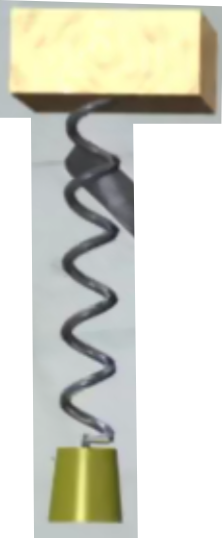
\includegraphics[scale = 0.30]{download(1)}
	\hspace{100pt}
	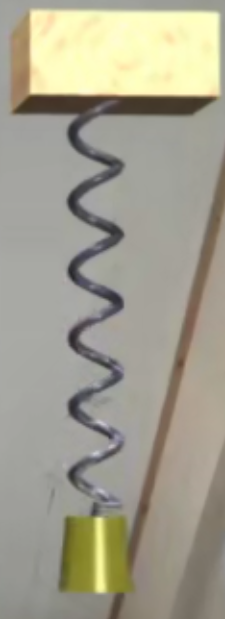
\includegraphics[scale = 0.35]{Screenshot (1480)}\\
\end{figure}

\begin{figure}[h]
	\centering
	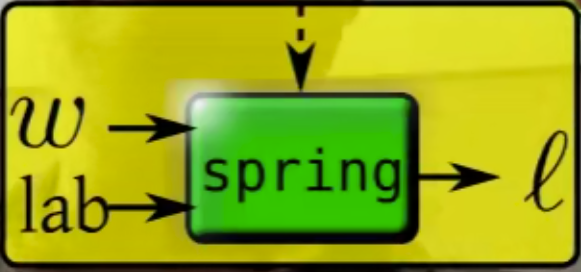
\includegraphics[scale = 0.5]{Screenshot (1479)}\\
\end{figure}

Observe that, here "lab" is a control factor. \\

For the springs from Lab 1 and Lab 2, we have the following weights as inputs and lengths as outputs respectively. \\
\begin{figure}[h]
	\centering
	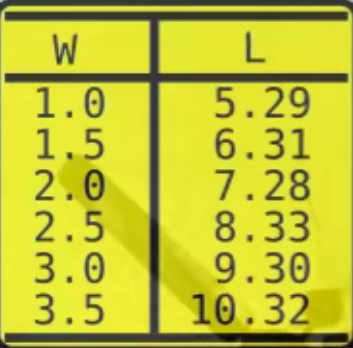
\includegraphics[scale = 0.5]{spring_lab_1}
	\hspace{100pt}
	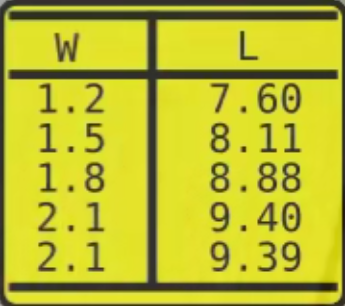
\includegraphics[scale = 0.5]{spring_lab_2}
\end{figure}

Now we shall load the two data sets in R.

\begin{knitrout}
\definecolor{shadecolor}{rgb}{0.969, 0.969, 0.969}\color{fgcolor}\begin{kframe}
\begin{alltt}
\hldef{data_lab_1} \hlkwb{=} \hlkwd{read.csv}\hldef{(}\hlsng{"springs_lab_1.csv"}\hldef{)}

\hldef{data_lab_1}
\end{alltt}
\begin{verbatim}
##   weight length
## 1    1.0   5.29
## 2    1.5   6.31
## 3    2.0   7.28
## 4    2.5   8.33
## 5    3.0   9.30
## 6    3.5  10.32
\end{verbatim}
\begin{alltt}
\hlkwd{dim}\hldef{(data_lab_1)}
\end{alltt}
\begin{verbatim}
## [1] 6 2
\end{verbatim}
\end{kframe}
\end{knitrout}

\begin{knitrout}
\definecolor{shadecolor}{rgb}{0.969, 0.969, 0.969}\color{fgcolor}\begin{kframe}
\begin{alltt}
\hldef{data_lab_2} \hlkwb{=} \hlkwd{read.csv}\hldef{(}\hlsng{"springs_lab_2.csv"}\hldef{)}

\hldef{data_lab_2}
\end{alltt}
\begin{verbatim}
##   weight length
## 1    1.2   7.60
## 2    1.5   8.11
## 3    1.8   8.88
## 4    2.1   9.40
## 5    2.1   9.39
\end{verbatim}
\begin{alltt}
\hlkwd{dim}\hldef{(data_lab_2)}
\end{alltt}
\begin{verbatim}
## [1] 5 2
\end{verbatim}
\end{kframe}
\end{knitrout}

We have to merge them to do operations.

\begin{knitrout}
\definecolor{shadecolor}{rgb}{0.969, 0.969, 0.969}\color{fgcolor}\begin{kframe}
\begin{alltt}
\hldef{temp_1} \hlkwb{=} \hlkwd{data.frame}\hldef{(data_lab_1,} \hlkwc{lab} \hldef{=} \hlnum{1}\hldef{)}

\hldef{temp_1}
\end{alltt}
\begin{verbatim}
##   weight length lab
## 1    1.0   5.29   1
## 2    1.5   6.31   1
## 3    2.0   7.28   1
## 4    2.5   8.33   1
## 5    3.0   9.30   1
## 6    3.5  10.32   1
\end{verbatim}
\begin{alltt}
\hldef{temp_2} \hlkwb{=} \hlkwd{data.frame}\hldef{(data_lab_2,} \hlkwc{lab} \hldef{=} \hlnum{2}\hldef{)}

\hldef{temp_2}
\end{alltt}
\begin{verbatim}
##   weight length lab
## 1    1.2   7.60   2
## 2    1.5   8.11   2
## 3    1.8   8.88   2
## 4    2.1   9.40   2
## 5    2.1   9.39   2
\end{verbatim}
\begin{alltt}
\hldef{all_data} \hlkwb{=} \hlkwd{rbind}\hldef{(temp_1, temp_2)}

\hldef{all_data}
\end{alltt}
\begin{verbatim}
##    weight length lab
## 1     1.0   5.29   1
## 2     1.5   6.31   1
## 3     2.0   7.28   1
## 4     2.5   8.33   1
## 5     3.0   9.30   1
## 6     3.5  10.32   1
## 7     1.2   7.60   2
## 8     1.5   8.11   2
## 9     1.8   8.88   2
## 10    2.1   9.40   2
## 11    2.1   9.39   2
\end{verbatim}
\end{kframe}
\end{knitrout}

Here, our model will be $$ l_{ij} = \alpha_i + \beta w_{ij} + \epsilon_{ij} $$
where $w_{ij}$ is the $j-th$ weight in $i-th$ lab. \\

For lab 1, we have a constant $\alpha_1$ and for lab 2, we have $\alpha_2$. \\

As the springs are almost identical, we have a constant $\beta$, same for both the springs. \\

Here, for $i=1$, $j=1(1)6$ and for $i=2$, $j=1(1)5$. \\

In matrix form, 
\begin{gather}
	\begin{bmatrix} l_{11} \\	l_{12} \\	\vdots \\	l_{16} \\ l_{21} \\ \vdots \\ l_{25}	\end{bmatrix}
	=
	\begin{bmatrix}	1 & 0 & w_{11} \\	1 & 0 & w_{12} \\	\vdots & \vdots & \vdots \\	1 & 0 & w_{16} \\ 0 & 1 & w_{21} \\ \vdots & \vdots & \vdots \\ 0 & 1 & w_{25} \end{bmatrix} 
	\cdot
	\begin{bmatrix}	\alpha_1 \\	\alpha_2 \\	\beta \\ \end{bmatrix}  
	+	
	\begin{bmatrix}  \epsilon_{11} \\	\epsilon_{12} \\	\vdots \\ \epsilon_{16} \\	\epsilon_{21} \\ \vdots \\ \epsilon_{25}	\end{bmatrix}.
\end{gather}


We have to change the "lab" to a factor. \\

\begin{knitrout}
\definecolor{shadecolor}{rgb}{0.969, 0.969, 0.969}\color{fgcolor}\begin{kframe}
\begin{alltt}
\hldef{all_data}\hlopt{$}\hldef{lab} \hlkwb{=} \hlkwd{factor}\hldef{(all_data}\hlopt{$}\hldef{lab)}
\end{alltt}
\end{kframe}
\end{knitrout}

\begin{knitrout}
\definecolor{shadecolor}{rgb}{0.969, 0.969, 0.969}\color{fgcolor}\begin{kframe}
\begin{alltt}
\hlkwd{class}\hldef{(all_data)}
\end{alltt}
\begin{verbatim}
## [1] "data.frame"
\end{verbatim}
\begin{alltt}
\hlkwd{class}\hldef{(all_data}\hlopt{$}\hldef{weight)}
\end{alltt}
\begin{verbatim}
## [1] "numeric"
\end{verbatim}
\begin{alltt}
\hlkwd{class}\hldef{(all_data}\hlopt{$}\hldef{length)}
\end{alltt}
\begin{verbatim}
## [1] "numeric"
\end{verbatim}
\begin{alltt}
\hlkwd{class}\hldef{(all_data}\hlopt{$}\hldef{lab)}
\end{alltt}
\begin{verbatim}
## [1] "factor"
\end{verbatim}
\end{kframe}
\end{knitrout}

\begin{knitrout}
\definecolor{shadecolor}{rgb}{0.969, 0.969, 0.969}\color{fgcolor}\begin{kframe}
\begin{alltt}
\hlkwd{plot}\hldef{(length} \hlopt{~} \hldef{weight, all_data,} \hlkwc{col} \hldef{= lab)}
\end{alltt}
\end{kframe}
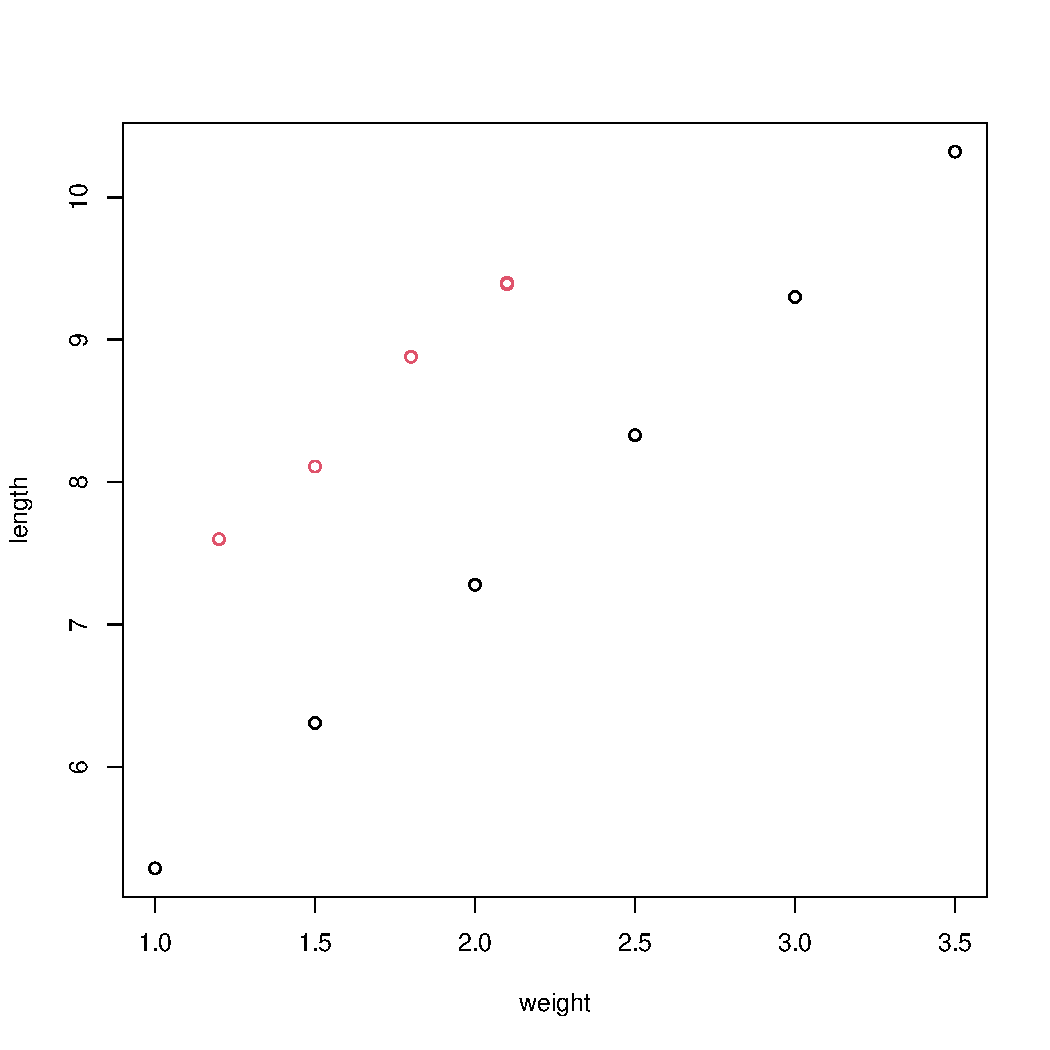
\includegraphics[width=\maxwidth]{figure/unnamed-chunk-21-1} 
\end{knitrout}

Now we shall fit our linear model.

\begin{knitrout}
\definecolor{shadecolor}{rgb}{0.969, 0.969, 0.969}\color{fgcolor}\begin{kframe}
\begin{alltt}
\hldef{fit_2} \hlkwb{=} \hlkwd{lm}\hldef{(length} \hlopt{~} \hldef{lab} \hlopt{+} \hldef{weight} \hlopt{-} \hlnum{1}\hldef{, all_data)}
\end{alltt}
\end{kframe}
\end{knitrout}

\begin{knitrout}
\definecolor{shadecolor}{rgb}{0.969, 0.969, 0.969}\color{fgcolor}\begin{kframe}
\begin{alltt}
\hldef{fit_2}
\end{alltt}
\begin{verbatim}
## 
## Call:
## lm(formula = length ~ lab + weight - 1, data = all_data)
## 
## Coefficients:
##   lab1    lab2  weight  
##  3.276   5.173   2.013
\end{verbatim}
\end{kframe}
\end{knitrout}

\begin{knitrout}
\definecolor{shadecolor}{rgb}{0.969, 0.969, 0.969}\color{fgcolor}\begin{kframe}
\begin{alltt}
\hlkwd{model.matrix}\hldef{(fit_2)}
\end{alltt}
\begin{verbatim}
##    lab1 lab2 weight
## 1     1    0    1.0
## 2     1    0    1.5
## 3     1    0    2.0
## 4     1    0    2.5
## 5     1    0    3.0
## 6     1    0    3.5
## 7     0    1    1.2
## 8     0    1    1.5
## 9     0    1    1.8
## 10    0    1    2.1
## 11    0    1    2.1
## attr(,"assign")
## [1] 1 1 2
## attr(,"contrasts")
## attr(,"contrasts")$lab
## [1] "contr.treatment"
\end{verbatim}
\end{kframe}
\end{knitrout}

\subsection*{2 Problems}

\begin{enumerate}

\item How to estimate $\beta$ when $\alpha_1$ and $\alpha_2$ are known ?
\item How to estimate $\beta$ and $\alpha_1$ when $\alpha_2$ is known ?

\end{enumerate}

\end{document}
